\begin{figure}
\caption{Hypothetical Scenarios of Error in the Measurement of Financial Market Stress at Elections Using an Annual Binary Measure vs. FinStress}
\label{election_timing_error}

\begin{subfigure}[b]{0.5\textwidth}
\centering
\caption{Time Order Measurement Error}

\resizebox{\linewidth}{!}{
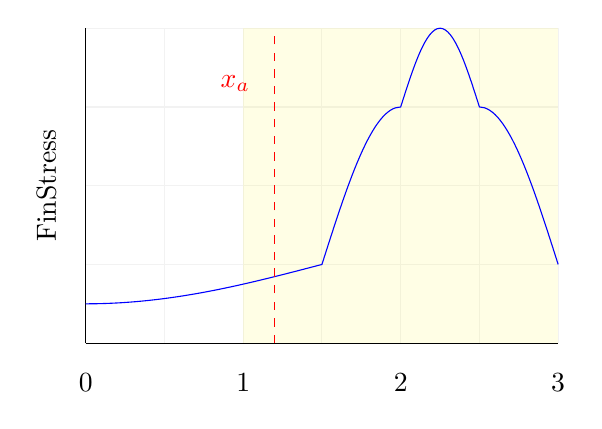
\begin{tikzpicture}

\node(t0) at (0,-0.5) {0};
\node(t1) at (2,-0.5) {1};
\node(t2) at (4,-0.5) {2};
\node(t3) at (6,-0.5) {3};

\node(yaxis)[rotate=90] at (-0.5, 2) {FinStress};

\draw[gray!10] (0,0) grid (6,4);

\draw[black] (0,0) -- (6,0);
\draw[black] (0,0) -- (0,4);

\fill[yellow, opacity=0.1] (2, 0) rectangle (6, 4);

\draw[blue] (0,0.5) cos (3, 1) sin (4,3) sin (4.5, 4) cos (5, 3) cos (6, 1);

\node(ax)[red] at (1.9, 3.3) {$x_{a}$};
\draw[red,dashed] (2.4, 0) -- (2.4, 4);

\end{tikzpicture}
}
\end{subfigure}
\begin{subfigure}[b]{0.5\textwidth}
\centering
\caption{Stress Intensity Measurement Error}

\resizebox{\linewidth}{!}{
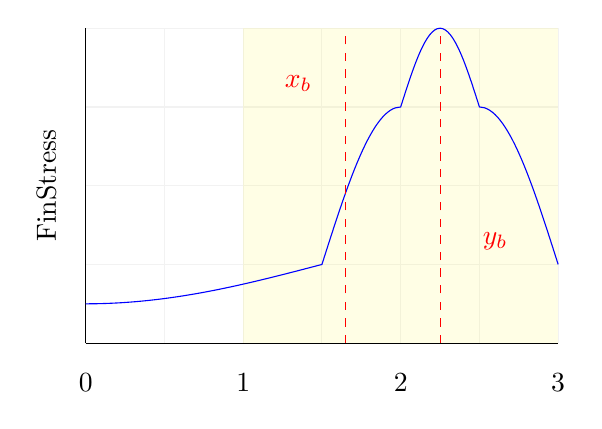
\begin{tikzpicture}

\node(t0) at (0,-0.5) {0};
\node(t1) at (2,-0.5) {1};
\node(t2) at (4,-0.5) {2};
\node(t3) at (6,-0.5) {3};

\node(yaxis)[rotate=90] at (-0.5, 2) {FinStress};

\draw[gray!10] (0,0) grid (6,4);

\draw[black] (0,0) -- (6,0);
\draw[black] (0,0) -- (0,4);

\fill[yellow, opacity=0.1] (2, 0) rectangle (6, 4);

\draw[blue] (0,0.5) cos (3, 1) sin (4,3) sin (4.5, 4) cos (5, 3) cos (6, 1);


\node(bx)[red] at (2.7, 3.3) {$x_{b}$};
\node(by)[red] at (5.2, 1.3) {$y_{b}$};

\draw[red,dashed] (3.3, 0) -- (3.3, 4);
\draw[red,dashed] (4.5, 0) -- (4.5, 4);

\end{tikzpicture}
}
\end{subfigure}

\begin{subfigure}[b]{0.5\textwidth}
\centering
\caption{Directional Change Measurement Issue}

\resizebox{\linewidth}{!}{
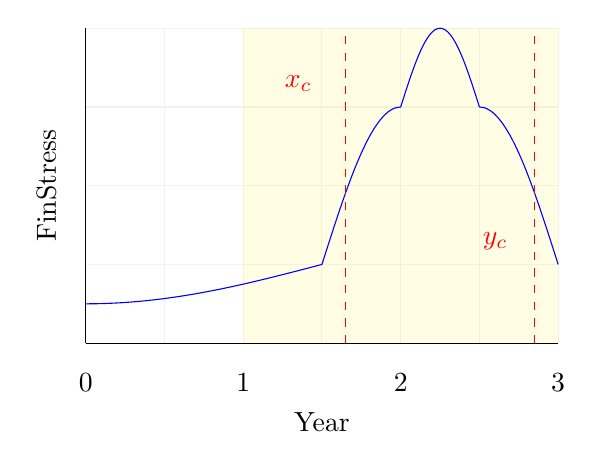
\begin{tikzpicture}

\node(t0) at (0,-0.5) {0};
\node(t1) at (2,-0.5) {1};
\node(t2) at (4,-0.5) {2};
\node(t3) at (6,-0.5) {3};

\node(xaxis) at (3, -1) {Year};
\node(yaxis)[rotate=90] at (-0.5, 2) {FinStress};

\draw[gray!10] (0,0) grid (6,4);

\draw[black] (0,0) -- (6,0);
\draw[black] (0,0) -- (0,4);

\fill[yellow, opacity=0.1] (2, 0) rectangle (6, 4);

\draw[blue] (0,0.5) cos (3, 1) sin (4,3) sin (4.5, 4) cos (5, 3) cos (6, 1);


\node(cx)[red] at (2.7, 3.3) {$x_{c}$};
\node(cy)[red] at (5.2, 1.3) {$y_{c}$};

\draw[red,dashed] (3.3, 0) -- (3.3, 4);
\draw[red,dashed] (5.7, 0) -- (5.7, 4);

\end{tikzpicture}
}
\end{subfigure}

{\scriptsize{
	Shaded area indicates years classified as a crisis by a binary crisis measure.
    Dashed vertical lines indicate an election.
}}

\end{figure}
